% !TEX root = ../../../main.tex
% 来源：中学数学实验教材·第一册（代数）
% 章节：多项式的四则运算 / 一元多项式的除法
% 原始文件：4.tex，行 2057-2066
% 类型：tikz
% ---
        \begin{tikzpicture}
      \node at (0,.5)[right]{$6+13+27+15$};
      \node at (4.5,.5){$-\tfrac{2}{3}$};
      \node at  (0,0) [right] {\quad $-4\;\; -6\;\; -14$};
      \node at (-.5, 0)[left]{$+)$};
      \draw (-1,-.25)--(4,-.25);
      \node at (0,-.75) [right]{$6\; +9\;+21 \quad \uwave{+1}$};
      \draw (4,-.25)--(4,1);
      \draw (4,.25)--(5,.25);
      \end{tikzpicture}  
